% !TeX root = ../tesis.tex


\section{Secciones transversales}
\label{section:yth}
La interacción luz–materia puede describirse clásicamente mediante dos procesos fundamentales: la absorción y el esparcimiento, cuyo efecto conjunto se denomina extinción del campo incidente. Experimentalmente, estos fenómenos se evidencian al comparar la potencia detectada con y sin la presencia de una partícula iluminada por un campo electromagnético incidente  ($\vb{E}_{\text{inc}}, \vb{H}_{\text{inc}}$) [ver Fig. \ref{scattering}] ~\cite{bohrenAbsorptionScatteringLight2008}.
%
\begin{figure}[h]
	\centering
	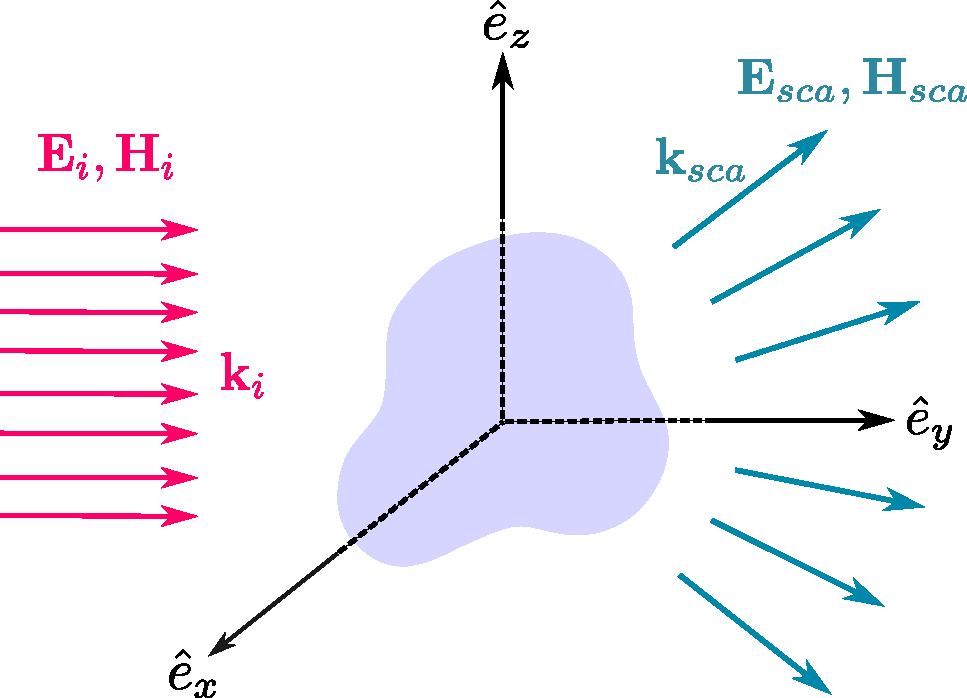
\includegraphics[width=8.5cm]{../../Figuras/scattering.pdf}
	\caption{Diagrama del problema de esparcimiento. El campo electromagnético ($\vb{E}_{\text{inc}}, \vb{H}_{\text{inc}}$) incide sobre una partícula arbitraria, produciendo el campo electromagnético esparcido ($\vb{E}_{\text{sca}}, \vb{H}_{\text{sca}}$).}
	\label{scattering}
\end{figure}
%
Para cuantificar este efecto de manera macroscópica, en esta sección se introducen las secciones transversales de extinción, absorción y esparcimiento, las cuales son cantidades macroscópicas medibles que proporcionan información sobre el sistema \cite{bohrenAbsorptionScatteringLight2008}. Para esto, se considera a la partícula embebida en un medio no absorbente e iluminada por una onda plana armónica en el tiempo~\cite{bohrenAbsorptionScatteringLight2008}. Teniendo en cuenta lo anterior, la energía transportada por los campos electromagnéticos y que es absorbida por la partícula $W_{\text{abs}}$, se calcula al integrar el promedio temporal del vector de Poynting\footnote{El promedio temporal del vector de Poynting es $\langle\vb{S}\rangle_t = (1/\tau)\int_t^{t+\tau}\vb{S}(t')\text{d}t'$, y para campos electromagnéticos del tipo ondas planas es $\langle\vb{S}\rangle_t = (1/2) \text{Re}[\vb{E} \times (\vb{B}/\mu)^{*}]$, donde $*$ denota la operación complejo conjugado \cite{bohrenAbsorptionScatteringLight2008}. } $\langle\vb{S}\rangle_t$  sobre una superficie cerrada $A$, que por simplificidad puede considerarse una esfera de radio $r$ mayor al de la partícula [ver Fig. \ref{WA}], es decir, 
\begin{tcolorbox}[ams align]
	W_{\text{abs}}=-\int_A \langle\vb{S}\rangle_t\cdot\vu{e}_r \text{ dA},
	\label{flujopoynting}
\end{tcolorbox}
\noindent donde, debido a que $\langle\vb{S}\rangle_t$ y $\vu{e}_r$ están orientados en la misma dirección, el signo negativo convierte a $W_{\text{abs}}$ en una cantidad positiva, de lo contrario, significaría que se genera energía dentro de la esfera \cite{bohrenAbsorptionScatteringLight2008}.
%
\begin{figure}[h]
	\centering
	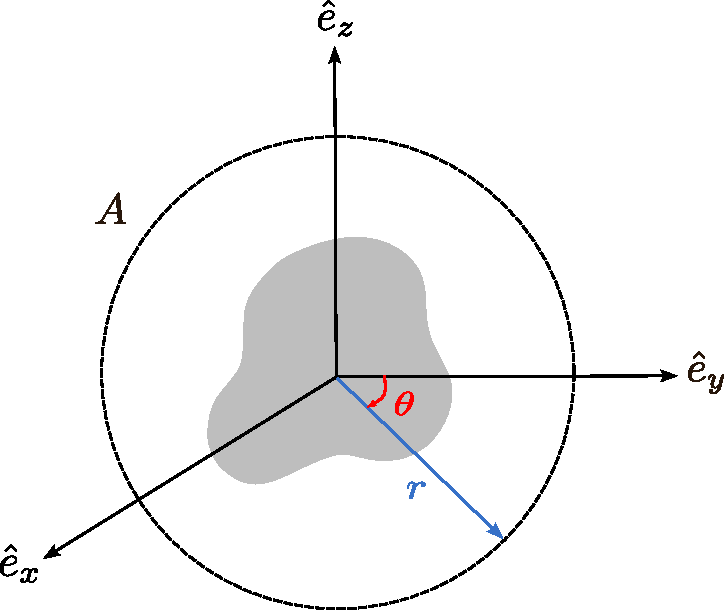
\includegraphics[width=7cm]{../../Figuras/WA.pdf}
	\caption{Esquema de la superficie de integración $A$ como una esfera de radio $r$ centrada en el origen y que contiene a la partícula de interés.}
	\label{WA}
\end{figure}
\\

\noindent Considerando la descomposición del vector de Poynting total en tres términos \cite{bohrenAbsorptionScatteringLight2008}
%
		
\begin{subequations}%
	\begin{tcolorbox}[
		ams align, breakable]
\langle\vb{S}^{\text{inc}}\rangle_t&=  \frac{1}{2}\:\mbox{Re}\{\vb{E}_{\text{inc}}\times\vb{H}_\text{inc}^*\},\\%
	\langle\vb{S}^{\text{sca}}\rangle_t&=  \frac{1}{2}\:\mbox{Re}\{\vb{E}_{\text{sca}}\times\vb{H}_{\text{sca}}^*\},\\%
	\langle\vb{S}^{\text{ext}}\rangle_t&= \frac{1}{2}\:\mbox{Re}\{\vb{E}_{\text{inc}}\times\vb{H}_{\text{sca}}^*+\vb{E}_{\text{sca}}\times\vb{H}_\text{inc}^*\},\label{eq:S}%
\end{tcolorbox}
\end{subequations}\vspace*{1em}
%

\noindent asociados al campo incidente, al campo esparcido y a la interacción entre los dos anteriores, respectivamente y donde Re$\{\cdot\}$ denota la parte real de un número complejo, se tiene que $W_{\text{abs}}=W_{\text{inc}}-W_{\text{sca}}+W_{\text{ext}}$, donde \cite{bohrenAbsorptionScatteringLight2008}
%
\begin{align} \label{eqs:W}
	W_{\text{inc}}  &= -\int_{A}\langle\vb{S}^{\text{inc}}\rangle_t\cdot\vu{e}_r\text{ dA},\label{Wi}\\ W_{\text{sca}}&=\int_{A}\langle\vb{S^{\text{sca}}}\rangle_t\cdot\vu{e}_r\text{ dA}, \label{Ws} \\ 
	W_{\text{ext}} &= -\int_{A}\langle\vb{S^{\text{ext}}}\rangle_t\cdot\vu{e}_r\text{ dA},\label{Wext} 
\end{align}
%
cuyos signos están colocados de forma que sean cantidades positivas considerando las direcciones de los vectores de Poynting y de $\vb{\hat{e}_r}$. En particular, para un medio no absorbente, la energía que cruza la esfera es la misma que la que entra, por lo que $W_{\text{inc}}$ se anula, entonces
%
\begin{equation}
	W_{\text{ext}}=W_{\text{abs}}+W_{\text{sca}}.
\end{equation}
%%

Al considerar el campo incidente $\vb{E}_{\text{inc}}=E\,\vu{e}_x$ y a $\vb{H}_{\text{inc}}=(1/\mu \omega)\: \vb{k} \times E\, \vu{e}_x$ en un medio no absorbente, $W_{\text{abs}}$ es independiente del radio $r$ de la superficie de integración, por lo que se puede considerar a $r$ lo suficientemente grande para estar en la región de campo lejano donde los campos se comportan como los generados por un dipolo inducido ($\vb{E}_p$, $\vb{H}_p$) al iluminar un sistema de cargas y corrientes con un onda electromagnética de frecuencia angular $\omega$ \cite{bohrenAbsorptionScatteringLight2008}
%
\begin{align}
	\vb{E}_{p}&=\frac{e^{ik(r-z)}}{-ikr}\vb{X}\:E_0 e^{ikz}\qquad\text{y}\qquad
	\vb{H}_{p}=\frac{k}{\omega\mu}\vu{e}_r\times\vb{E}_{p},
	\label{EH_s}
\end{align}
%
donde $\vb{X}$ es el vector de amplitud de esparcimiento dado por
\begin{equation}
	\vb{X}=\frac{ik^3}{4\pi}\alpha \left[ \vu{e}_r\times(\vu{e}_r\times \vu{e}_x)\right]=\frac{ik^3}{4\pi}\alpha \left(-\cos\theta\cos\phi\, \vu{e}_{\theta}+\sin\phi\, \vu{e}_{\phi} \right),
	\label{eq:Xvec}
\end{equation}
%
por lo cual, $W_{\text{ext}}$ está dado por \cite{bohrenAbsorptionScatteringLight2008}
%
\begin{equation*}
	W_{\text{ext}}=I_i\frac{4\pi}{k^2}\:\text{Re}\{(\vb{X}\cdot\vu{e}_x)_{\theta=0}\}
\end{equation*}
%
y además, $I_{\text{inc}}$ es la irradiancia de la onda incidente, que corresponde a la magnitud del vector de Poynting, y por consiguiente\footnote{Debido al teorema óptico, la extinción sólo depende de la amplitud de esparcimiento en la dirección de propagación y es el efecto combinado de la absorción en la partícula y el esparcimiento por la partícula en todas las direcciones \cite{bohrenAbsorptionScatteringLight2008}.},
%
\begin{equation}
	C_{\text{ext}}=\frac{W_{\text{ext}}}{I_i}=\frac{4\pi}{k^2}\:\text{Re}\{(\vb{X}\cdot\vu{e}_x)_{\theta=0}\}, \label{C_ext}
\end{equation}
%
que es la sección transversal de extinción y que posee dimensiones de área. La Ec. (\ref{C_ext}) puede ser reescrita como \cite{bohrenAbsorptionScatteringLight2008}
%
\begin{tcolorbox}[ams align]
	C_{\text{ext}}=C_{\text{abs}}+C_{\text{sca}},
	\label{C} 
\end{tcolorbox}
%
\noindent donde $C_{\text{abs}}=W_{\text{abs}}/I_{\text{inc}}$ y $C_{\text{sca}}=W_{\text{sca}}/I_{\text{inc}}$ corresponden a las secciones transversales de absorción y esparcimiento, respectivamente. Al sustituir las Ecs. (\ref{EH_s}) en la Ec. (\ref{Ws}) se obtiene
%
\begin{equation}
	C_{\text{sca}}=\int_0^{2\pi}\int_0^{\pi}\frac{|\vb{X}|^2}{k^2}\:\sin\theta\: \text{d}\theta\:\text{d}\phi.
	\label{C_sca_general}
\end{equation}
%%
Las Ecs. (\ref{C_ext})--(\ref{C_sca_general}) son propiedades macroscópicas y medibles que proveen información sobre la energía absorbida y esparcida por una partícula.  \\

